\documentclass[a4paper]{article}
\usepackage[utf8]{inputenc}
\usepackage{array}
\usepackage{graphicx}
\usepackage{geometry}
\usepackage{tabularx}
\usepackage{float}
\usepackage{xcolor,listings}
\usepackage{textcomp}
\usepackage{hyperref}
% \UseRawInputEncoding

\newcommand\YAMLcolonstyle{\color{red}\mdseries}
\newcommand\YAMLkeystyle{\color{black}\bfseries}
\newcommand\YAMLvaluestyle{\color{blue}\mdseries}

\makeatletter

% here is a macro expanding to the name of the language
% (handy if you decide to change it further down the road)
\newcommand\language@yaml{yaml}

\expandafter\expandafter\expandafter\lstdefinelanguage
\expandafter{\language@yaml}
{
  keywords={true,false,null,y,n},
  keywordstyle=\color{darkgray}\bfseries,
  basicstyle=\YAMLkeystyle,                                 % assuming a key comes first
  sensitive=false,
  comment=[l]{\#},
  morecomment=[s]{/*}{*/},
  commentstyle=\color{purple}\ttfamily,
  stringstyle=\YAMLvaluestyle\ttfamily,
  moredelim=[l][\color{orange}]{\&},
  moredelim=[l][\color{magenta}]{*},
  moredelim=**[il][\YAMLcolonstyle{:}\YAMLvaluestyle]{:},   % switch to value style at :
  morestring=[b]',
  morestring=[b]",
  literate =    {---}{{\ProcessThreeDashes}}3
                {>}{{\textcolor{red}\textgreater}}1     
                {|}{{\textcolor{red}\textbar}}1 
                {\ -\ }{{\mdseries\ -\ }}3,
}

% switch to key style at EOL
\lst@AddToHook{EveryLine}{\ifx\lst@language\language@yaml\YAMLkeystyle\fi}
\makeatother

\newcommand\ProcessThreeDashes{\llap{\color{cyan}\mdseries-{-}-}}

\definecolor{codepurple}{HTML}{C42043}

 \geometry{
 a4paper,
 total={130mm,257mm},
 %left=20mm,
 top=25mm,
 bottom=25mm
 }

\graphicspath{ {./images/} }
% \newcolumntype{L}[1]{>{\arraybackslash}m{#1}}
\newcolumntype{L}[1]{>{\raggedright\let\newline\\\arraybackslash\hspace{1pt}}m{#1}}

\title{Progetto di Basi di Dati - Sito Cinema e TV}
\author{Samuele Pecetto}
\date{\today}

\begin{document}
\maketitle
\newpage
\tableofcontents
\newpage

\section{Progettazione concettuale}
\filbreak
\subsection{Requisiti iniziali}

Si veda il documento \emph{esame\_progettazione\_requisiti.pdf} contenente l'analisi funzionale del progetto.\\

\subsection{Glossario dei termini}

% \begin{center}

\begin{tabular}{ L{0.17\textwidth} L{0.43\textwidth} L{0.15\textwidth} L{0.20\textwidth} }
% \begin{tabular}{l l l l }
\\
\hline
\textbf{Termine} & \textbf{Descrizione} & \textbf{Sinonimi} & \textbf{Collegamenti} \\
\hline
\hline

 Redattore & Utente responsabile del caricamento e aggiornamento dei contenuti disponibili sulla piattaforma & Utente redazione & Contenuto, Metadati \\ 
 
\hline
Metadati & Informazioni inserite dai redattori, relative ai contenuti come Titolo, Paese, Genere, Data di uscita ecc. & dati dei Film, Serie, ecc & Contenuto, Redattore \\

\hline
 Visitatore & Utente registrato capace di votare e/o aggiungere ai propri preferiti, contenuti pubblicati dai redattori & Utente & Preferiti, Voto \\ 
 
\hline
 Voto & Votazione espressa con un numero naturale compreso tra 1 e 5 da un utente Visitatore per un contenuto & Votazione & Contenuto, Utente, Visitatore \\
 
\hline
 Preferiti & Insieme di contenuti che il Visitatore può registrare nella sua area personale &  & Visitatore \\
 
\hline
 Contenuti & Insieme di risorse cinematografiche & Film, Serie, Episodi, Programmi &  \\  
 
\hline
 Piattaforma & Mezzo di trasmissione dei contenuti - Streaming, canali DTV &  & Serie, Programmi \\
 
\hline
 Sito & Sito internet dell'applicazione tipo Coming Soon & Sito Cinema e TV &  \\
 
\hline
 Personaggio & Individuo appartenente al mondo dello spettacolo. Vengono considerati Personaggi i Registi,
 Sceneggiatori, Attori, Fotografi, Musicisti e più in generale chiunque partecipi attivamente alla realizzazione di 
 contenuti cinematografici &  & Contenuto \\
 
 \hline
 Fotografo & Abbreviazione del più preciso Direttore della fotografia & Direttore della fotografia & Contenuto, Personaggio \\

\hline
 Interpretazione & Nome del soggetto di fantasia interpretato dal personaggio nel contenuto specificato & & Personaggio, Attore \\ 
 
\hline
 Indirizzo & Aggregazione di Paese, Provincia, Città, Indirizzo e Civico di un luogo & Luogo Nascita & Cinema \\

 \hline
 Contatti & Metodi di contatto come numeri di telefono e/o indirizzi email & Contatti telefonici & Cinema \\
\end{tabular}
% \end{center}

\filbreak
\subsection{Requisiti rivisti e strutturati in gruppi di frasi omogenee}

Si vuole realizzare una base di dati per la gestione di una sito che fornisce
informazioni su contenuti cinematografici come film, serie TV e programmi TV, ispirato a siti internet come 
ComingSoon.\\
I redattori sono utenti responsabili dell' aggiornamento dei
contenuti e metadati disponibili sul sito come Film, Serie TV e relativi Episodi, Programmi TV.\\
I redattori sono responsabili dell'inserimento delle programmazioni delle proiezioni dei Film nelle sale dei
 cinema per ogni contenuto disponibile sul sito.\\
I redattori sono responsabili dell'inserimento delle programmazioni televisive per i contenuti disponibili sul sito.\\
Sul sito possono registrarsi degli utenti visitatori che possono aggiungere nei loro preferiti e votare i contenuti presenti sul sito.
Per i visitatori e per i redattori si devono memorizzare username, password e email.\\
Per i redattori si deve memorizzare anche la data di inizio collaborazione.\\
I contenuti hanno una serie di metadati da memorizzare che consistono di:
Titolo, Descrizione, Data di uscita, Genere, Anno, Registi, Attori con relativa interpretazione, 
Paese, Durata, Distributori, Sceneggiatori, Fotografi, Musicisti e Produttori.\\
Ogni serie TV è composta da una o più stagioni.\\
Ogni stagione è composta da uno o più episodi, dei quali si devono memorizzare specifici metadati 
che consistono di: Titolo, Registi, Attori, Sceneggiatori, Durata.\\
Per ogni personaggio si deve memorizzare: Nome, Foto, Biografia, Contenuti in cui ha partecipato,
 Data e luogo di nascita.\\
I film vengono proiettati nei cinema. Per ogni cinema si deve memorizzare: Nome, 
Contatti telefonici, Indirizzo.\\
Di ogni proiezione si deve memorizzare: Data e ora, Sala del cinema, Prezzo del biglietto. \\
Programmi e Serie TV vanno in onda su canali TV o piattaforme di streaming video, 
dove vengono organizzate per genere.\\

\subsection{Schema E-R + business rules}
\begin{center}
\begin{figure}[h]
  \makebox[\textwidth]{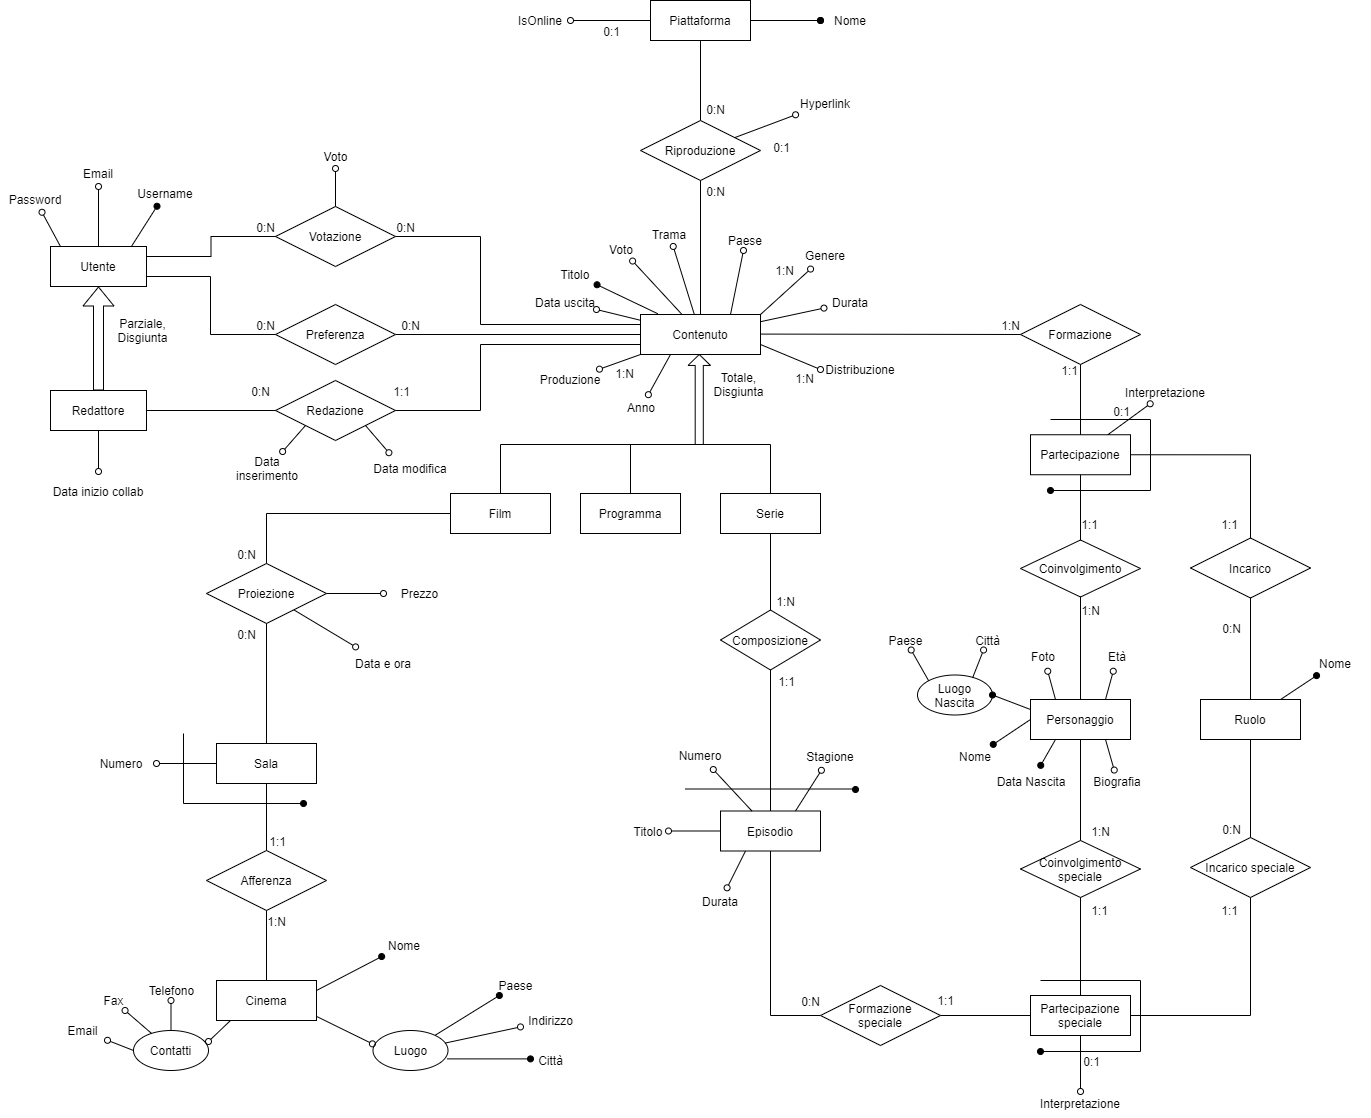
\includegraphics[width=1.45\textwidth]{Coming-soon-er-Iniziale.png}}
  \caption{Schema ER iniziale}
  \end{figure}
\end{center}

\clearpage
Osserviamo che l'identificatore primario delle entità deboli Partecipazione e Partecipazione speciale includono 
l'attributo opzionale Interpretazione, in quanto si vuole supportare la casistica in cui un Personaggio può
far parte del cast di un Contenuto con svariati ruoli, oltre che come attore di diverse interpretazioni.
Si pensi ad esempio a un film di Carlo Verdone dove interpreta diversi personaggi ed è anche regista dei suoi film.\\
Essendo però illegale la definizione di una chiave primaria composita con attributi opzionali, nella fase di ristrutturazione
verrà introdotto un identificatore numerico sequenziale per ovviare al problema, permettendo la definizione di tuple
che altrimenti creerebbero violazione di chiave, negli scenari appena descritti.\\\\
{\large \textbf{Regole di vincolo}}
\begin{itemize}
  \item L'attributo Voto dell'associazione Votazione tra Utente e Contenuto è un numero naturale compreso tra 1 e 5.
  \item L'attributo Interpretazione dell'entità Partecipazione/Partecipazione speciale deve essere valorizzato soltanto 
  nelle istanze con ruolo pari ad Attore.
  \item L'attributo Hyperlink dell'associazione tra Contenuto e Piattaforma può essere valorizzato solo nel caso in cui la Piattaforma sia online.
  \item L'attributo Data modifica dell'associazione Redazione tra Redattore e Contenuto deve essere strettamente maggiore della Data inserimento.
  % \item L'aggiunta di episodi ad una serie deve essere sequenziale: 1 -2 -3 ma non 2- 1 - 3 ecc
\end{itemize}

\hfill \break
{\large \textbf{Regole di derivazione}}
\begin{itemize}
  \item La Votazione di un contenuto è ottenuta facendo la media aritmetica dei voti per quel contenuto di tutti gli utenti. 
  \item L'anno di un contenuto è ottenuto estraendo l'anno dalla data di uscita.
  \item Il cast di default di un Episodio è desumibile dal cast associato alla Serie di appartenenza.
\end{itemize}


\clearpage
\section{Progettazione logica}
\subsection{Tavola dei volumi}

\hfill \break
Si suppone che ogni serie abbia mediamente 2 stagioni di cui ognuna composta da 8 episodi. \\
Si suppone che ogni episodio che ha specifici attori, registi e sceneggiatori, siano 
già partecipanti ad altri contenuti (non vanno a modificare la cardinalità di Personaggi). \\
Si suppone che Piattaforma contenga oltre ai siti di streaming ($10$), anche i canali TV ($40$). \\
Si suppone che mediamente per ogni contenuto ci siano $5$ attori con ruoli principali di cui si 
vuole tenere traccia. \\
Si suppone che mediamente ogni attore partecipi a $5$ contenuti. \\
Si suppone che mediamente ci sia $1$ regista per ogni contenuto. \\
Si suppone che mediamente ogni regista partecipi a $10$ contenuti. \\
Si suppone che mediamente ci siano $2$ sceneggiatori per ogni contenuto. \\
Si suppone che mediamente ogni sceneggiatore partecipi a $10$ contenuti. \\
Si suppone che mediamente ci sia $1$ fotografo per ogni contenuto. \\
Si suppone che mediamente ogni fotografo partecipi a $20$ contenuti. \\
Si suppone che mediamente ci sia $1$ musicista per ogni contenuto. \\
Si suppone che mediamente ogni musicista partecipi a $50$ contenuti. \\
Si suppone che mediamente ogni $10$ episodi di una serie ci siano 
$1$ regista, $1$ attore, $1$ sceneggiatore, $1$ musicista e $1$ fotografo diversi
rispetto a quelli della serie stessa. \\
Si suppone che mediamente ogni cinema abbia $2$ sale. \\
Si suppone che ogni utente voti mediamente 50 contenuti diversi. \\ 
Si suppone che ogni utente aggiunga ai preferiti mediamente 5 contenuti diversi. \\
Si suppone che ogni contenuto venga mediamente riprodotto su 5 piattaforme diverse. \\
Si suppone che ogni film venga riprodotto 2 volte in un cinema. \\

\begin{tabular}{ | L{0.33\textwidth} | L{0.33\textwidth} | L{0.33\textwidth} | }

\hline
\textbf{Concetto} & \textbf{Tipo} & \textbf{Volume} \\

\hline
% entità
\hline
 Utente & E & $10000$ \\ 
 
\hline
 Redattore & E & $100$ \\ 
 
\hline
 Contenuto & E & $100000$ \\ 
 
\hline
 Partecipazione & E & $1000000$ \\ 
 
\hline
 Partecipazione speciale & E & $160000$ \\ 
 
\hline
 Ruolo & E & $5$ \\ 
 
\hline
 Film & E & $50000$ \\ 
 
\hline
 Programma & E & $30000$ \\ 
 
\hline
 Serie & E & $20000$ \\ 
 
\hline
 Episodio & E & $320000$ \\
 
\hline
 Piattaforma & E & $50$ \\ 
 
\hline
 Personaggio & E & $47000$ \\ 
 
\hline
 Sala & E & $600$ \\ 
 
\hline
 Cinema & E & $300$ \\ 
% associazioni 
\hline
 Votazione & R & $500000$ \\ 

\hline
 Preferenza & R & $50000$ \\ 

\hline
 Redazione & R & $100000$ \\ 

\hline
 Riproduzione & R & $500000$ \\ 

\hline
 Composizione & R & $320000$ \\ 

\hline
 Proiezione & R & $30000000$ \\ 

\hline
 Afferenza & R & $600$ \\ 

 \hline
 Formazione & R & $1000000$ \\ 

\hline
Formazione speciale & R & $160000$ \\ 

\hline
 Coinvolgimento & R & $1000000$ \\ 

\hline
Coinvolgimento speciale & R & $160000$ \\ 

\hline
 Incarico & R & $1000000$ \\ 

\hline
Incarico speciale & R & $160000$ \\ 

\hline
\end{tabular}
\\

\subsection{Tavola delle operazioni}
Basandoci sulla regola dell'\emph{80-20}, consideriamo le operazioni di seguito 
elencate come le più costose, in termini di esecuzione e frequenti. \\
In particolare, il criterio di scelta delle seguenti operazioni è veicolato dalle \\
entità e relazioni con il maggior numero di tuple coinvolte, che 
risultano essere quelle delle proiezioni e delle partecipazioni dei personaggi a contenuti. \\
Inoltre, si assume che lo scopo principale del sito sia quello di fornire capacità agli utenti
di visualizzare metadati dei loro film/attori preferiti. Questo porta a scegliere prevalentemente
operazioni interattive. \\

\hfill \break

\begin{tabular}{ | L{0.63\textwidth} | L{0.13\textwidth} | L{0.23\textwidth} | }

\hline
\textbf{Operazione} & \textbf{Tipo} & \textbf{Frequenza} \\

\hline
\hline
Registrazione nuovo Utente & I & 20 / giorno \\

\hline
Redazione nuovo contenuto & I & 20 / giorno \\

\hline
Ricerca contenuto & I & 5000 / giorno \\

\hline
Ricerca personaggio & I & 5000 / giorno \\

\hline
Visualizzazione scheda contenuto & I & 5000 / giorno \\

\hline
Visualizzazione scheda personaggio & I & 5000 / giorno \\

\hline
Votazione di un contenuto & I & 500 / giorno \\

\hline
Ricerca di proiezioni disponibili per un film & I & 500 / giorno \\ 

\hline
Aggiornamento media delle votazioni di un contenuto & B & 500 / giorno \\ 

\hline

\end{tabular}

\begin{quotation}\footnotesize
\textbf{I:} Interattiva \quad \textbf{B:} Batch
\end{quotation}

\subsection{Ristrutturazione schema E-R}
\subsubsection{Analisi delle ridondanze}
\textbf{Attributo Voto}\\
Nell'attuale formalizzazione si possono riscontrare delle ridondanze nell'attributo Voto presente
in Contenuto. \\
Infatti il valore medio si può estrarre tramite interrogazione nell'associazione Votazione tra Utente 
e Contenuto. 
\begin{center}
\begin{figure}[h]
  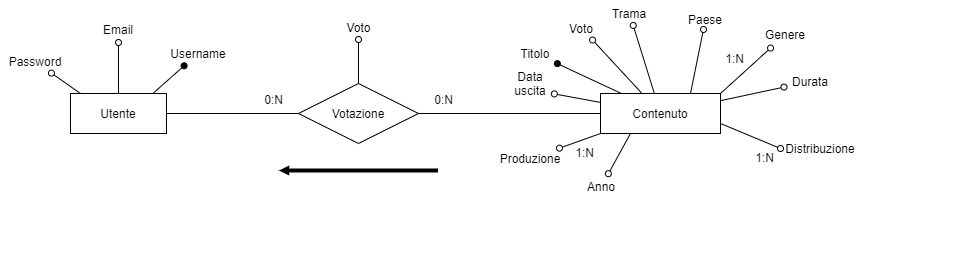
\includegraphics[width=1.2\textwidth]{Coming-soon-er-Sliced.png}
  \caption{Schema di navigazione}
\end{figure}
\end{center}

Considerando pessimisticamente che un contenuto riceve mediamente 5 voti, sono necessari 5 accessi in lettura 
nella relazione Votazione per determinarne la media. 

\begin{table}[H]
\begin{tabular}{ | l | l | l | l | }
\hline
\textbf{Concetto} & \textbf{Costrutto} & \textbf{Accessi} & \textbf{Tipo} \\
\hline
\hline
Contenuto & Entità & 1 & R \\
\hline
\end{tabular}
  \caption{Tavola degli accessi dell'operazione Visualizzazione scheda contenuto \textbf{con ridondanza}}
\end{table}

\begin{table}[H]
\begin{tabular}{ | l | l | l | l | }
\hline
\textbf{Concetto} & \textbf{Costrutto} & \textbf{Accessi} & \textbf{Tipo} \\
\hline
\hline
Votazione & Relazione & 4 & R \\
Votazione & Relazione & 1 & W \\
Contenuto & Entità & 1 & W \\
\hline
\end{tabular}
  \caption{Tavola degli accessi dell'operazione votazione contenuto \textbf{con ridondanza}}
\end{table}

\begin{table}[H]
\begin{tabular}{ | l | l | l | l | }
\hline
\textbf{Concetto} & \textbf{Costrutto} & \textbf{Accessi} & \textbf{Tipo} \\
\hline
\hline
Contenuto & Entità & 1 & R \\
\hline
Votazione & Relazione & 5 & R \\
\hline
\end{tabular}
  \caption{Tavola degli accessi dell'operazione Visualizzazione scheda contenuto \textbf{senza ridondanza}}
\end{table}

\begin{table}[H]
\begin{tabular}{ | l | l | l | l | }
\hline
\textbf{Concetto} & \textbf{Costrutto} & \textbf{Accessi} & \textbf{Tipo} \\
\hline
\hline
Votazione & Relazione & 1 & W \\
\hline
\end{tabular}
  \caption{Tavola degli accessi dell'operazione votazione contenuto \textbf{senza ridondanza}}
\end{table}

\begin{quotation}\footnotesize
\textbf{R:} Read \quad \textbf{W:} Write 
\end{quotation}

Dal punto di vista della memoria l'attributo Voto in contenuto dovendo contenere un numero float (real) compreso tra 1 e 5, occuperà 
4 bytes di spazio, che sono decisamente trascurabili. ($ 4 \cdot 100000 = 0,4 Megabytes $)\\
Nello scenario con la ridondanza si ha l'operazione di Visualizzazione contenuto trascurabile, mentre l'operazione 
di votazione più pesante da mantenere in quanto richiede la lettura delle precedenti votazioni per quello stesso contenuto.\\
D'altro canto senza ridondanza l'operazione più pesante diventa quella del calcolo della media voti, mentre l'operazione di votazione 
è trascurabile. \\
Considerando però che il numero di visualizzazioni giornaliere della scheda contenuti (5000) è nettamente superiore 
a quella delle votazioni (500) (oltre alla sottostima di soli 5 voti per contenuto, nella realtà sono sicuramente di più) 
si decide di mantenere la ridondanza, che verrà aggiornata tramite trigger in seguito a una votazione che avverrà con meno frequenza.\\
Accessi totali giornalieri con ridondanza: \\
\begin{center}
Visualizzazione scheda contenuto: \quad $ 5000 \cdot 1 = 5000 $ \\
Votazione: \quad $ 500 \cdot (4 + ( 1 \cdot 2) + ( 1 \cdot 2)) = 4000 $ \\
Totale: \quad $ 5000 + 4000  = 9000 $ \\
\end{center}
Accessi totali giornalieri senza ridondanza: \\
\begin{center}
Visualizzazione scheda contenuto: \quad $ 5000 \cdot 6 = 30000 $ \\
Votazione: \quad $ 500 \cdot ( 1 \cdot 2) = 1000 $ \\
Totale: \quad $ 30000 + 1000 = 31000 >> 9000$ \\
\end{center}
\textbf{Partecipazione / Partecipazione speciale}\\
Un'altra ridondanza è rappresentata dall'associazione Partecipazione (reificata in entità) su Contenuto e Partecipazione 
speciale (reificata in entità) su Episodio.\\
Episodio essendo collegato alla entità Serie, eredita le associazioni di Contenuto. \\
In questo caso possiamo esplicitare una funzione diversa per le 2 associazioni
che permettono di preservare la copertura delle funzionalità richieste e nel contempo di eliminare la ridondanza. \\
In particolare, possiamo considerare l'associazione Partecipazione tra Contenuto e Personaggio come 
la definizione del Cast di default, mentre l'associazione Partecipazione speciale tra Episodio e Personaggio 
può essere vista come un override del cast, che contiene soltanto le eccezioni per un determinato episodio. \\
In questo modo non sarà necessario specificare per ogni episodio tutto il cast, dato che verrà desunto dalla serie di appartenenza.
Tale operazione sarà necessaria in caso di eccezioni, con un considerevole risparmio di inserimento di tuple. \\
\textbf{Attributo Anno}\\
Una ulteriore ridondanza è rappresentata dall'attributo Anno in Contenuto. Infatti l'anno di pubblicazione 
di un contenuto può essere desunto ed estratto tramite funzioni sql dalla data di pubblicazione.
Data la semplicità di estrazione e la mancanza di valore aggiunto si decide di rimuovere la ridondanza. \\
\textbf{Attributo Età}\\
La medesima considerazione si può fare per l'attributo Età in Personaggio dato che può essere agevolmente calcolata
a partire dalla data odierna.
Data la semplicità di estrazione e la mancanza di valore aggiunto si decide di rimuovere la ridondanza. \\

\subsubsection{Eliminazione delle generalizzazioni}
Le generalizzazioni presenti nell'attuale schema ER sono: Utente (parziale e disgiunta) con un sottoinsieme Redattore e 
Contenuto (totale e disgiunta) formata dai sottoinsiemi Film, Serie TV e Programma.\\

\subsubsection{Partizionamento/Accorpamento di entità e associazioni}
In entrambi i casi si decide di tradurre le generalizzazioni con l'accorpamento delle entità figlie 
nel padre.\\
Gli svantaggi principali dati da questo design consistono principalmente nello spreco di memoria, dato che 
gli attributi specifici delle entità figlie non vengono valorizzati quando l'occorrenza è di tipo diverso, risultando 
in valori null.\\
In entrambi i casi lo spreco di memoria è irrisorio dato che gli attributi aggiuntivi sono rispettivamente:\\
\begin{itemize}
  \item Data inizio e fine collaborazione per Redattore \\
\item Un unico attributo \emph{Tipo}, atto a determinare la tipologia di ogni istanza di Contenuto.\\
\end{itemize}
A tal proposito, l'attributo Tipo è sufficiente, in quanto la generalizzazione è disgiunta. Non sono quindi
contemplati casi in cui un Film è anche Programma Tv o una Serie è anche un Film, ecc.\\
Tale soluzione garantisce inoltre minori accessi e quindi migliori prestazioni per funzionalità (operazioni)
come ricerca di contenuti senza specificarne il tipo.\\
Nel caso degli utenti invece, non è necessario aggiungere l'attributo tipo per identificare i redattori, in quanto l'informazione
può essere desunta controllando il valore dell'attributo Data inizio collaborazione. \\
Per sopperire al caso in cui un redattore interrompa le sue prestazioni di lavoro, introduciamo un ulteriore attributo \emph{Data fine collaborazione}
che permette di non dover cancellare le informazioni relative all'utenza e di mantenere lo storico delle sue redazioni di 
schede contenuto.\\
Con tale modifica, per determinare se un utente è un redattore piuttosto che un visitatore, sarà sufficiente verificare che 
data inizio collaborazione abbia un valore (passato) e che data fine collaborazione non abbia valore (o valore futuro). \\
\subsubsection{Scelta degli identificatori principali}
Per poter risolvere le inefficienze legate all'utilizzo di chiavi composte,
chiavi alfanumeriche particolarmente lunghe o chiavi con identificatori esterni,
sono stati introdotti i seguenti identificatori principali:
\begin{itemize}
  \item Id per l'associazione Votazione (supporto cancellazione utente)\\ 
  \item Id per l'associazione Redazione (supporto cancellazione utente)\\ 
  \item Id per l'entità Sala \\
  \item Id per l'entità Cinema \\
  \item Id per l'entità Episodio\\
  \item Id per l'entità Personaggio\\
  \item Id per l'entità Contenuto\\
  \item Id per l'entità Piattaforma\\
  \item Id per l'entità Partecipazione\\
  \item Id per l'entità Partecipazione speciale\\
\end{itemize}

Si decide di mantenere Username come chiave di Utente in quanto si ipotizza di creare delle regole di business
che ne vincolino la composizione come caratteri consentiti e lunghezza minima / massima.\\
\subsection{Schema E-R ristrutturato + business rules}
\begin{center}
\begin{figure}[h]
  \makebox[\textwidth]{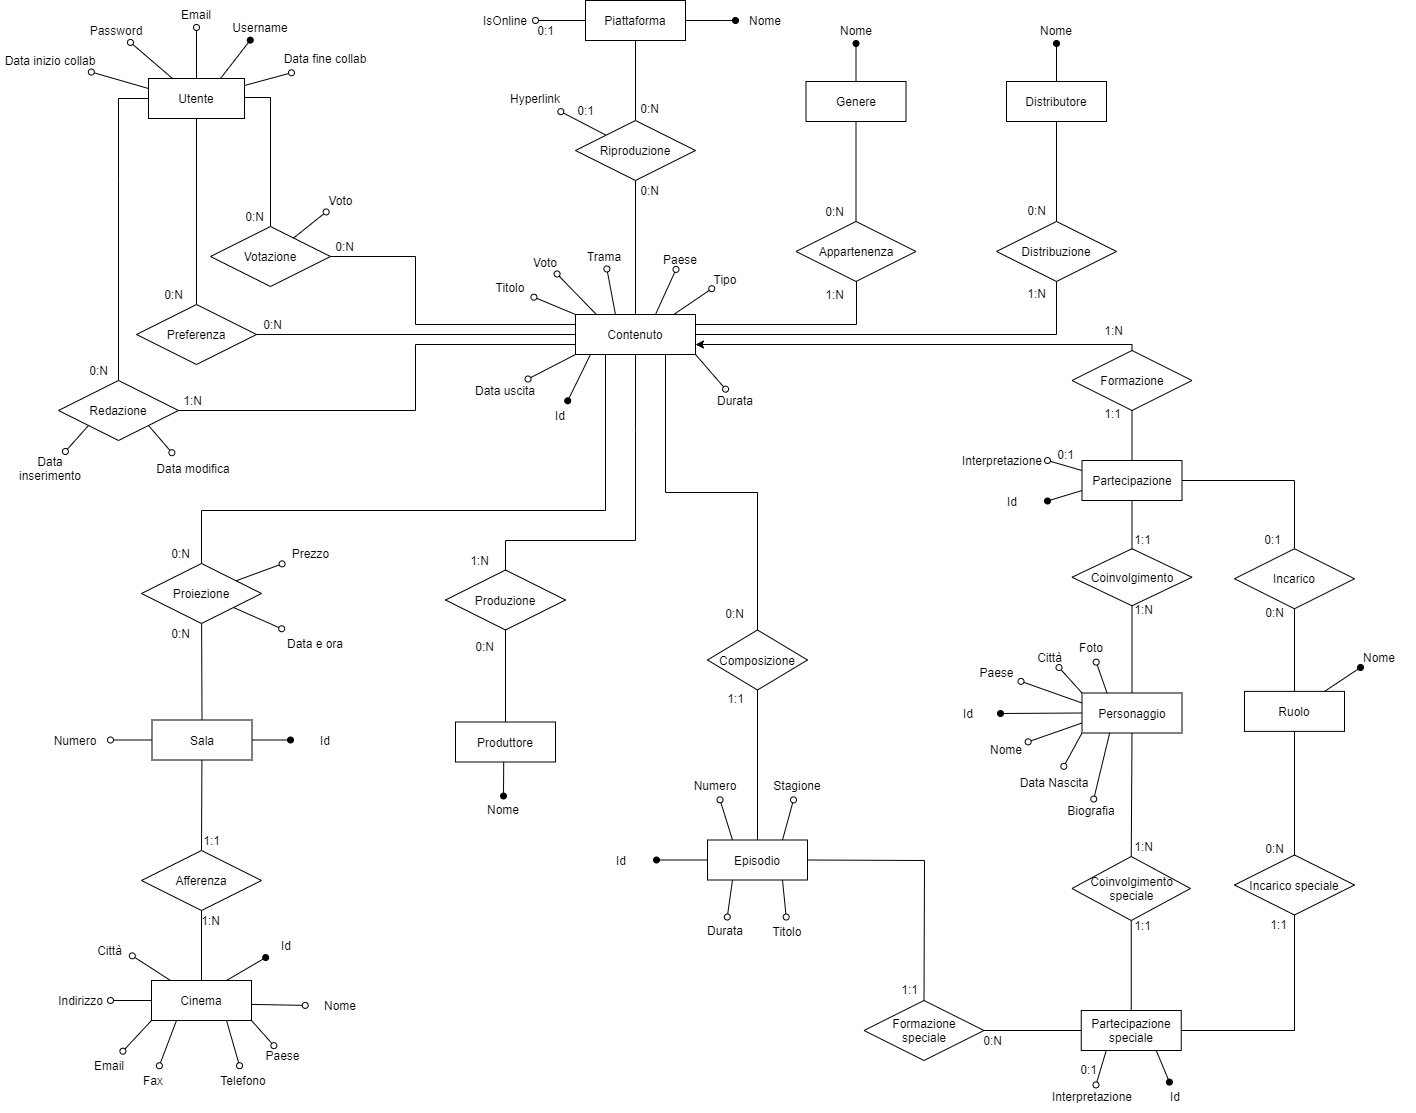
\includegraphics[width=1.45\textwidth]{Coming-soon-er-Ristrutturato.png}}
  \caption{Schema ER Ristrutturato}
  \end{figure}
\end{center}

Le business rules sono le medesime già definite nel capitolo 1 più la seguente:\\
{\large \textbf{Regole di vincolo}}
\begin{itemize}
  \item Un contenuto può essere proiettato in un cinema soltanto se è di tipo Film.\\
\end{itemize}

\subsection{Schema relazionale}
Lo schema ER ristrutturato viene tradotto nelle seguenti relazioni:\\\\
\textbf{utente}(\underline{username}, email, password, data\_inizio\_collaborazione, data\_fine\_collaborazione)\\
\textbf{contenuto}(\underline{id}, titolo, voto, trama, paese, data\_uscita, tipo, durata)\\
\textbf{partecipazione}(\underline{id}, id\_contenuto, id\_personaggio, ruolo, interpretazione)\\
\textbf{partecipazione\_speciale}(\underline{id}, id\_episodio, id\_personaggio, ruolo, interpretazione)\\
\textbf{ruolo}(\underline{nome})\\
\textbf{piattaforma}(\underline{nome}, is\_online)\\
\textbf{genere}(\underline{nome})\\
\textbf{distributore}(\underline{nome})\\
\textbf{personaggio}(\underline{id}, biografia, data\_nascita, nome, paese, città, foto)\\
\textbf{episodio}(\underline{id}, serie, numero, stagione, durata, titolo)\\
\textbf{produttore}(\underline{nome})\\
\textbf{sala}(\underline{id}, numero, id\_cinema)\\
\textbf{cinema}(\underline{id}, nome, paese, email, telefono, fax, indirizzo, città)\\
\textbf{contenuto\_votazione}(\underline{id}, id\_contenuto, username, voto)\\
\textbf{contenuto\_preferenza}(\underline{id\_contenuto, username})\\
\textbf{contenuto\_redazione}(\underline{id}, id\_contenuto, username, data\_inserimento, data\_modifica)\\
\textbf{contenuto\_riproduzione}(\underline{id\_contenuto, piattaforma}, hyperlink)\\
\textbf{contenuto\_genere}(\underline{id\_contenuto, genere})\\
\textbf{contenuto\_distribuzione}(\underline{id\_contenuto, distributore})\\
\textbf{contenuto\_produzione}(\underline{id\_contenuto, produttore})\\
\textbf{contenuto\_proiezione}(\underline{id\_contenuto, id\_sala, data\_ora}, prezzo)\\

{\large \textbf{Vincoli di integrità referenziale (in "dot notation"):}}\\
\begin{itemize}
  \item id\_contenuto in partecipazione referenzia contenuto.id;\\
  \item id\_personaggio in partecipazione referenzia personaggio.id;\\
  \item ruolo in partecipazione referenzia ruolo.nome;\\
  \item id\_episodio in partecipazione\_speciale referenzia episodio.id;\\
  \item id\_personaggio in partecipazione\_speciale referenzia personaggio.id;\\
  \item ruolo in partecipazione\_speciale referenzia ruolo.nome;\\
  \item id\_cinema in sala referenzia cinema.id;\\
  \item id\_contenuto in contenuto\_votazione referenzia contenuto.id;\\
  \item username in contenuto\_votazione referenzia utente.username;\\
  \item id\_contenuto in contenuto\_preferenza referenzia contenuto.id;\\
  \item username in contenuto\_preferenza referenzia utente.username;\\
  \item id\_contenuto in contenuto\_redazione referenzia contenuto.id;\\
  \item username in contenuto\_redazione referenzia utente.username;\\
  \item id\_contenuto in contenuto\_riproduzione referenzia contenuto.id;\\
  \item piattaforma in contenuto\_riproduzione referenzia piattaforma.nome;\\
  \item id\_contenuto in contenuto\_genere referenzia contenuto.id;\\
  \item genere in contenuto\_genere referenzia genere.nome;\\
  \item id\_contenuto in contenuto\_distribuzione referenzia contenuto.id;\\
  \item distributore in contenuto\_distribuzione referenzia distributore.nome;\\
  \item id\_contenuto in contenuto\_produzione referenzia contenuto.id;\\
  \item produttore in contenuto\_produzione referenzia produttore.nome;\\
  \item id\_contenuto in contenuto\_proiezione referenzia contenuto.id;\\
  \item id\_sala in contenuto\_proiezione referenzia sala.id;\\
\end{itemize}


\begin{quotation}\footnotesize
  Si decide di adottare come naming convention (per omogeneità con l'implementazione sql) per relazioni (tabelle) 
  e attributi \emph{lowercase separato da underscore}
  in riferimento al fatto che, citando la documentazione ufficiale 
  "Key words and unquoted identifiers are case insensitive."\\
  Si decide inoltre di denominare le relazioni risultanti da associazioni molti a molti con la seguente struttura:
  {nome entità soggetto}\_{nome associazione}, quando il nome dell'associazione è autoesplicativo e sufficiente
  a interpretare la relazione intuitivamente.\\
  Nel caso particolare di Contenuto - Appartenenza - Genere, si decide invece di adottare contenuto\_genere.\\
  La scelta di anteporre il nome dell'entità soggetto è voluta, per semplificare la ricerca e l'uso pratico 
  della base dati.\\
  source: \url{https://www.postgresql.org/docs/current/sql-syntax-lexical.html#SQL-SYNTAX-IDENTIFIERS}
\end{quotation}
\clearpage
\section{Implementazione}
L'ambiente di sviluppo viene creato tramite un container docker tramite docker-compose di cui si 
allega il file descrittore :
\lstinputlisting[
  language=yaml,
  showspaces=false,
  basicstyle=\ttfamily,
  numbers=left,
  numberstyle=\tiny,
  breaklines=true,
  showstringspaces=false
  ]
{postgres/docker-compose.yml}

\subsection{DDL: Creazione del Database}

\lstinputlisting[
  language=SQL,
  showspaces=false,
  basicstyle=\ttfamily,
  numbers=left,
  numberstyle=\tiny,
  commentstyle=\color{gray},
  keywordstyle=\color{codepurple},
  breaklines=true,
  showstringspaces=false
  ]
{postgres/schema.sql}

\subsection{DML: Popolamento tabelle}
\lstinputlisting[
  language=SQL,
  showspaces=false,
  basicstyle=\ttfamily,
  numbers=left,
  numberstyle=\tiny,
  commentstyle=\color{gray},
  keywordstyle=\color{codepurple},
  breaklines=true,
  showstringspaces=false
  ]
{postgres/data.sql}

\subsection{Contraints check: Operazioni di cancellazione e modifica}
\lstinputlisting[
  language=SQL,
  showspaces=false,
  basicstyle=\ttfamily,
  numbers=left,
  numberstyle=\tiny,
  commentstyle=\color{gray},
  keywordstyle=\color{codepurple},
  breaklines=true,
  showstringspaces=false
  ]
{postgres/checks.sql}

\end{document}
